\section{How to Create Plots?}

We will now show several possibilities for plotting, using different
technologies. For each of the following technologies, we give an example to
provide an idea to the reader of how the work with this technology might look
like. The examples are in alphabetical order of the technology name; afterwards
we will only look closer into \texttt{pgfplots}.

\subsection{GNUplot}

\subsection{pgfplots}

\subsection{PSTricks}

\subsection{R and Sweave}

\begin{listing}[H]
  \inputminted{latex}{../examples/sweave-example.Snw}
  \caption{Plot the exchange rate between \euro{} and \$ dynamically using
    Sweave}
  \label{lst:sweave-example}
\end{listing}
\begin{figure}[t]
  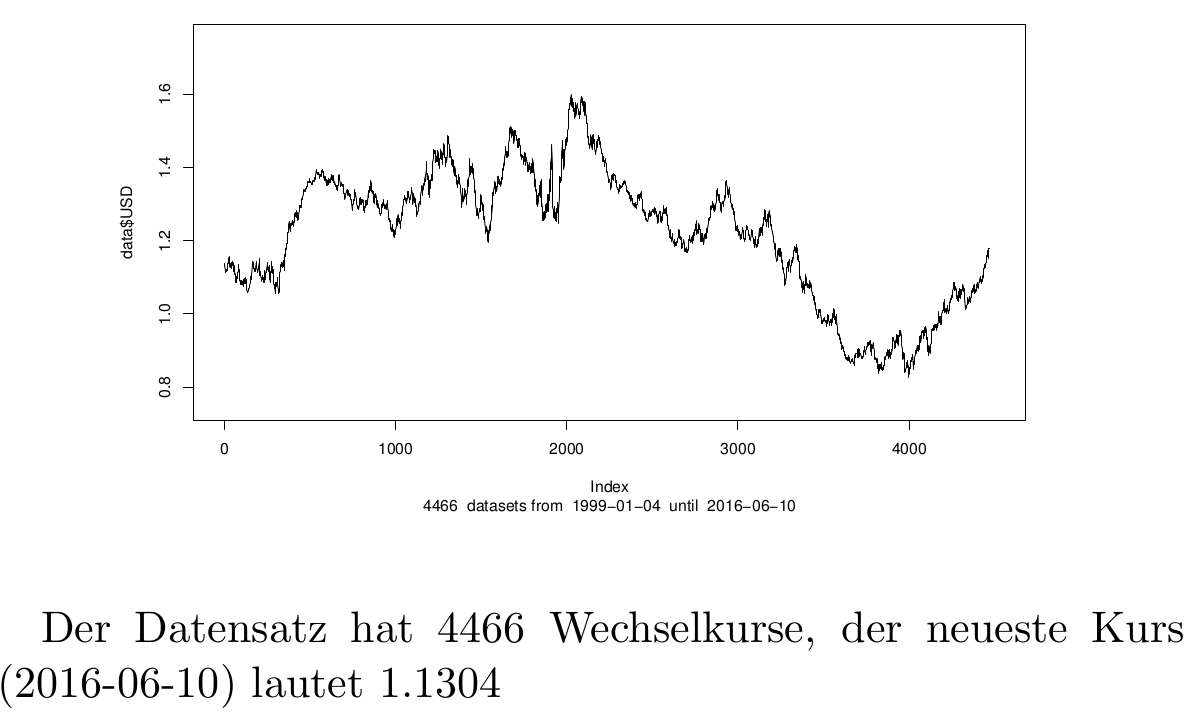
\includegraphics[width=\linewidth]{sweave-example}
  \caption{Screenshot of the Sweave example in Lst.~\ref{lst:sweave-example}}
  \label{fig:sweave-example}
\end{figure}
